%%%
%% This is file `sample-sigplan.tex',
%% generated with the docstrip utility.
%%
%% The original source files were:
%%
%% samples.dtx  (with options: `sigplan')
%%
%% IMPORTANT NOTICE:
%%
%% For the copyright see the source file.
%%
%% Any modified versions of this file must be renamed
%% with new filenames distinct from sample-sigplan.tex.
%%
%% For distribution of the original source see the terms
%% for copying and modification in the file samples.dtx.
%%
%% This generated file may be distributed as long as the
%% original source files, as listed above, are part of the
%% same distribution. (The sources need not necessarily be
%% in the same archive or directory.)
%%
%%
%% Commands for TeXCount
%TC:macro \cite [option:text,text]
%TC:macro \citep [option:text,text]
%TC:macro \citet [option:text,text]
%TC:envir table 0 1
%TC:envir table* 0 1
%TC:envir tabular [ignore] word
%TC:envir displaymath 0 word
%TC:envir math 0 word
%TC:envir comment 0 0
%%
%%
%% The first command in your LaTeX source must be the \documentclass command.
%%\documentclass[sigplan,nonacm]{acmart}
%%\documentclass[sigplan, nonacm]{acmart}\settopmatter{printfolios=true,printccs=false,printacmref=false}
\documentclass[acmsmall,nonacm]{acmart}\settopmatter{printfolios=true,printccs=false,printacmref=false}

\graphicspath{{pictures/}}
%%
%% \BibTeX command to typeset BibTeX logo in the docs
\AtBeginDocument{%
	\providecommand\BibTeX{{%
			\normalfont B\kern-0.5em{\scshape i\kern-0.25em b}\kern-0.8em\TeX}}}

%% Rights management information.  This information is sent to you
%% when you complete the rights form.  These commands have SAMPLE
%% values in them; it is your responsibility as an author to replace
%% the commands and values with those provided to you when you
%% complete the rights form.
%%\setcopyright{acmcopyright}
\setcopyright{none}
%%\acmJournal{PACMPL}
%%\acmVolume{1}
%%\acmNumber{CONF} % CONF = POPL or ICFP or OOPSLA
%%\acmArticle{1}
%%\acmYear{2021}
%%\acmMonth{9}
%%\acmDOI{}
%%\copyrightyear{2018}
%%\acmYear{2018}
%%\acmDOI{10.1145/1122445.1122456}

%% These commands are for a PROCEEDINGS abstract or paper.
%%\acmConference[Woodstock '18]{Woodstock '18: ACM Symposium%% on Neural
%%  Gaze Detection}{June 03--05, 2018}{Woodstock, NY}
%%\acmBooktitle{Woodstock '18: ACM Symposium on Neural Gaze Detection,
%%  June 03--05, 2018, Woodstock, NY}
%%\acmPrice{15.00}
%%\acmISBN{978-1-4503-XXXX-X/18/06}


%%
%% Submission ID.
%% Use this when submitting an article to a sponsored event. You'll
%% receive a unique submission ID from the organizers
%% of the event, and this ID should be used as the parameter to this command.
%%\acmSubmissionID{123-A56-BU3}

%%
%% The majority of ACM publications use numbered citations and
%% references.  The command \citestyle{authoryear} switches to the
%% "author year" style.
%%
%% If you are preparing content for an event
%% sponsored by ACM SIGGRAPH, you must use the "author year" style of
%% citations and references.
%% Uncommenting
%% the next command will enable that style.
%%\citestyle{acmauthoryear}
\usepackage{xspace}
\usepackage{booktabs}   %% For formal tables:
                        %% http://ctan.org/pkg/booktabs
\usepackage{subcaption} %% For complex figures with subfigures/subcaptions
                        %% http://ctan.org/pkg/subcaption

\usepackage[utf8]{inputenc}
\usepackage[T1]{fontenc}
\usepackage[scaled=0.78]{beramono}
\usepackage{amsmath}
\usepackage{mathtools}
\usepackage{stmaryrd}
%\usepackage{unicode-math}
%\usepackage{MnSymbol}
\usepackage{wasysym}
\usepackage{color}
\usepackage{xcolor,colortbl}
\usepackage{url}
\usepackage{listings}
\usepackage{paralist}
%\usepackage[compact]{titlesec}
\usepackage[font={small}]{caption}
\usepackage{wrapfig}
\usepackage{enumitem}
\usepackage{multicol}
\usepackage{multirow}
\usepackage{makecell}
\usepackage{flushend}
\usepackage{bcprules}
\usepackage{textcomp}
\usepackage{tikz}
\usetikzlibrary{positioning,fit,calc,arrows.meta,arrows,decorations}
\usepackage{pdfpages}
\usepackage{cleveref}
\usetikzlibrary{matrix}
\usepackage{xspace}
\definecolor{light-gray}{gray}{0.85}
\usepackage{stackengine}
\usepackage{mathpartir}
\usepackage{float}
% ----- listings

%\definecolor{ckeyword}{HTML}{7F0055}
\definecolor{ckeyword}{HTML}{000000}
\definecolor{ccomment}{HTML}{3F7F5F}
\definecolor{cstring}{HTML}{2A0099}

\lstdefinelanguage{Scala}%
{morekeywords={
  abstract, sealed, lazy,
  case,catch,char,class,%
  def,do,else,extends,final,finally,for,%
  if,import,implicit,%
  match,module,%
  new,null,undefined,%
  %fun,
  array,
  override,%
  package,private,protected,public,%
  for,public,return,super,%
  this,throw,trait,try,type,%
  val,var,%
  with,while,%
  object,
  let,skip,assert,then,fst,snd,idx,sum,prod,exists,forall,%
  yield,%
  % some scheme keywords
  define, null?, car, cdr
  },%
  sensitive,%
  moredelim=*[il][\bfseries]{\#\#\ },
  morecomment=[l]//,%
  morecomment=[s]{/*}{*/},%
  morestring=[b]",%
  %morestring=[b]',%
  showstringspaces=false%
}[keywords,comments,strings]%

\lstdefinelanguage{Effect}%
{morekeywords={
    effect, yield, return
  },%
  sensitive,%
  moredelim=*[il][\bfseries]{\#\#\ },
  morecomment=[l]//,%
  morecomment=[s]{/*}{*/},%
  morestring=[b]",%
  %morestring=[b]',%
  showstringspaces=false%
}[keywords,comments,strings]%

\lstdefinelanguage{LLVM}%
{morekeywords={
    define, i32, br, icmp, sub, call, mul, phi, ret, label
  },%
  sensitive,%
  moredelim=*[il][\bfseries]{\#\#\ },
  morecomment=[l];,%
  morecomment=[s]{/*}{*/},%
  morestring=[b]",%
  %morestring=[b]',%
  showstringspaces=false%
}[keywords,comments,strings]%

\lstdefinelanguage{CPP}%
{morekeywords={
    using, void, function, if, else, Cont, List
  },%
  sensitive,%
  moredelim=*[il][\bfseries]{\#\#\ },
  morecomment=[l]//,%
  morecomment=[s]{/*}{*/},%
  morestring=[b]",%
  %morestring=[b]',%
  showstringspaces=false%
}[keywords,comments,strings]%


\lstset{
  language=Scala,%
  mathescape=true,%
%  columns=[c]fixed,%
  aboveskip=2pt,%\smallskipamount,
  belowskip=1pt,%\negsmallskipamount,
  lineskip=-1pt,
  basewidth={0.6em, 0.5em},%
%  backgroundcolor=\color{listingbg},
  basicstyle=\ttfamily,
  keywordstyle=\keywordstyle,
  commentstyle=\commentstyle,
  stringstyle=\stringstyle,
%  xleftmargin=0.5cm
  literate={-->}{{$\to$}}2
           {->}{{$\mapsto$}}3
           {<-}{{$\leftarrow$}}2
           {=>}{{$\Rightarrow ~$}}2
           {|-}{{$\ts$}}2
           %{fun}{{$\lambda$}}1
           {idx}{{$\#$}}1
           {array(}{{$\langle.\rangle$(}}3
           {σ}{{$\sigma$}}1
           {ρ}{{$\rho$}}1
           {→}{{$\to$}}1
           {←}{{$\leftarrow$}}1
           {λ}{{$\lambda$}}1
           {α}{{$\alpha$}}1
           {⊔}{{$\sqcup$}}1
           {⊓}{{$\sqcap$}}1
           {⊑}{{$\sqsubseteq$}}1
           {⊤}{{$\top$}}1
           {⊥}{{$\bot$}}1
           {×}{{$\times$}}1
           {τ}{{$\tau$}}1
           {ψ}{{$\psi$}}1
           {Σ}{{$\Sigma$}}1
           {⟨}{{$\langle$}}1
           {⟩}{{$\rangle$}}1
           {π}{{$\pi$}}1
           {∪}{{$\cup$}}2
           %{[[}{{$[\![$}}1
           %{]]}{{$]\!]$}}1
           %{…}{{$\!...$}}1
}

\lstdefinestyle{small}{
  language=Scala,%
  mathescape=true,%
%  columns=[c]fixed,%
  aboveskip=2pt,%\smallskipamount,
  belowskip=1pt,%\negsmallskipamount,
  lineskip=-1pt,
  basewidth={0.6em, 0.45em},%
%  backgroundcolor=\color{listingbg},
  basicstyle=\fontsize{7}{9}\selectfont\ttfamily,
  keywordstyle=\keywordstyle,
  commentstyle=\commentstyle,
  stringstyle=\stringstyle,
%  xleftmargin=0.5cm
  literate={-->}{{$\to$}}3
           {->}{{$\mapsto$}}3
           {=>}{{$\Rightarrow ~$}}2
           {|-}{{$\ts$}}2
           %{fun}{{$\lambda$}}1
           {idx}{{$\#$}}1
           {sum}{{$\Sigma$}}1
           {array(}{{$\langle.\rangle$(}}3
           {σ}{{$\sigma$}}1
           {ρ}{{$\rho$}}1
           {→}{{$\to$}}1
           {λ}{{$\lambda$}}1
           {α}{{$\alpha$}}1
           {⊔}{{$\sqcup$}}1
           {⊓}{{$\sqcap$}}1
           {⊑}{{$\sqsubseteq$}}1
           {⊤}{{$\top$}}1
           {⊥}{{$\bot$}}1
           {×}{{$\times$}}1
           {τ}{{$\tau$}}1
           {ψ}{{$\psi$}}1
           %{[[}{{$[\![$}}1
           %{]]}{{$]\!]$}}1
           %{…}{{$\!...$}}1
}

\lstdefinestyle{extrasmall}{
  language=Scala,%
  mathescape=true,%
%  columns=[c]fixed,%
  aboveskip=2pt,%\smallskipamount,
  belowskip=1pt,%\negsmallskipamount,
  lineskip=-1pt,
  basewidth={0.6em, 0.45em},%
%  backgroundcolor=\color{listingbg},
  basicstyle=\fontsize{6}{8}\selectfont\ttfamily,
  keywordstyle=\keywordstyle,
  commentstyle=\commentstyle,
  stringstyle=\stringstyle,
%  xleftmargin=0.5cm
  literate={-->}{{$\to$}}3
           {->}{{$\mapsto$}}3
           {=>}{{$\Rightarrow ~$}}2
           {|-}{{$\ts$}}2
           %{fun}{{$\lambda$}}1
           {idx}{{$\#$}}1
           {sum}{{$\Sigma$}}1
           {array(}{{$\langle.\rangle$(}}3
           {σ}{{$\sigma$}}1
           {ρ}{{$\rho$}}1
           {→}{{$\to$}}1
           {λ}{{$\lambda$}}1
           {α}{{$\alpha$}}1
           {⊔}{{$\sqcup$}}1
           {⊓}{{$\sqcap$}}1
           {⊑}{{$\sqsubseteq$}}1
           {⊤}{{$\top$}}1
           {⊥}{{$\bot$}}1
           {×}{{$\times$}}1
           %{[[}{{$[\![$}}1
           %{]]}{{$]\!]$}}1
           %{…}{{$\!...$}}1
}

\lstdefinestyle{JavaScriptTiny}{
    style=JavaScript, % Inherit from the JavaScript style
    basicstyle=\ttfamily\tiny,
    numberstyle=\ttfamily\tiny, % Set the number style to \tiny
}

\lstdefinestyle{JavaScript}{
    language=java,
    basicstyle=\ttfamily\scriptsize,
    keywordstyle=\color{blue},
    commentstyle=\color{green!50!black},
    stringstyle=\color{black},
    showstringspaces=false,
    breaklines=true,
    breakatwhitespace=true,
    tabsize=1,
    numbersep=2pt,
    numberstyle=\ttfamily\tiny,
    % morekeywords={let, const, var, function, if, else, pipe, map, group, count, plus, minus,
    % while, for, return, typeof, switch, case, merge, get, sum, min, max, div, keyval, apply, times},
    morekeywords={let, const, var, function, if, else}
    escapeinside={(*@}{@*)}
}

\lstdefinestyle{JavaScriptInline}{
    language=java,
    basicstyle=\ttfamily\scriptsize,
    keywordstyle=\color{blue},
    commentstyle=\color{green!50!black},
    stringstyle=\color{black},
    showstringspaces=true,
    breaklines=true,
    breakatwhitespace=true,
    tabsize=1,
    numbersep=2pt,
    numberstyle=\ttfamily\tiny,
    morekeywords={},
    escapeinside={(*@}{@*)}
}

\lstset{style=JavaScript, upquote=true}

\lstdefinestyle{JSComment}{
    language=java,
    basicstyle=\color{green!50!black}\ttfamily\scriptsize,
    commentstyle=\color{green!50!black},
    showstringspaces=true,
    breaklines=true,
    breakatwhitespace=true,
    tabsize=1,
}

\definecolor{listingbg}{RGB}{240, 240, 240}

\newcommand{\commentstyle}[1]{\color{ccomment}\itshape{#1}}
\newcommand{\keywordstyle}[1]{\color{ckeyword}\bfseries{#1}}
%\newcommand{\keywordstyle}[1]{\color{ckeyword}{#1}}
%\newcommand{\stringstyle}[1]{\color{cstring}\bfseries{#1}}
\newcommand{\stringstyle}[1]{\color{cstring}\text{#1}}

\lstnewenvironment{listing}{\lstset{language=Scala}}{}
\lstnewenvironment{listingtiny}{\lstset{language=Scala,basicstyle=\scriptsize\ttfamily}}{}

\newcommand{\code}[1]{\lstinline[language=Scala,columns=fixed,basicstyle=\ttfamily]|#1|}

% ----- packed items, so we don't waste space
\newenvironment{sitemize}{
\begin{itemize}[leftmargin=2.5ex]
  \setlength{\itemsep}{1pt}
  \setlength{\parskip}{0pt}
  \setlength{\parsep}{0pt}
}{\end{itemize}}

\newenvironment{senumerate}{
\begin{enumerate}[leftmargin=2.5ex]
  \setlength{\itemsep}{1pt}
  \setlength{\parskip}{0pt}
  \setlength{\parsep}{0pt}
}{\end{enumerate}}

\newcommand{\mypar}[1]{{\bf #1.}}

% ----- formal

%\newcommand{\judgement}[2]{{\bf #1} \hfill #2}
%\newcommand{\den}[1]{$\left\llbracket$\;#1\;$\right\rrbracket$}
\newcommand{\den}[1]{\llbracket~#1~\rrbracket}

%\newcommand{\ts}{\,\vdash\,}
\newcommand{\evalsto}{\Downarrow}

\newcommand{\mbind}{\;{\small{\texttt{>>}\hspace{-0.3pt}\raisebox{-0.15pt}{\texttt{=}}}}\;}

%\newcommand{\mbind}{{\small{\texttt{>>}\hspace{-1.7pt}\raisebox{-0.15pt}{\texttt{=}}}}}

\newcommand{\rref}[1]{\textsc{(#1)}}

% ----- comments and todo

\newcommand{\note}[1]{{\color{red}[#1]}}
\newcommand{\snote}[1]{{\color{blue}[#1]}}
\newcommand{\todo}[1]{\note{TODO: #1}}
\newcommand{\rev}[1]{\note{Revision: #1}}

\newcommand{\silent}[1]{}

\newcommand{\hl}[1]{\setlength{\fboxsep}{0pt}\colorbox{light-gray}{#1}}

%\newcommand{\SECFork}{\textsc{sec}$_{\pitchfork}$}
\newcommand{\SECFork}{\textsc{sec}$_{{\mathrlap{<}-}}$}
\newcommand{\SECConc}{\textsc{sec}$_v$}
\newcommand{\SECBack}{\textsc{sec}$_{\hookleftarrow}$}
\newcommand{\inline}[1]{\lstinline[style=JavaScriptInline,basicstyle=\ttfamily\small]{#1}}
\newcommand{\highlight}[2][yellow]{\setlength{\fboxsep}{1pt}\colorbox{#1}{#2}}



%%
%% end of the preamble, start of the body of the document source.
\newcommand{\rhyme}{\text{Rhyme}\xspace}
\newcommand{\ul}[1]{\underline{#1}}
\newcommand{\lb}{\{~}
\newcommand{\rb}{~\}}

\newcommand{\Typ}[1]{\ensuremath{\mathsf{#1}}}
\newcommand{\Ast}[1]{\ensuremath{\textsf{\text{#1}}}}
\newcommand{\Def}[1]{\ensuremath{\mathrm{#1}}}
\newcommand{\mit}[1]{\ensuremath{\mathit{#1}}}
\newcommand{\msf}[1]{\ensuremath{\mathsf{#1}}}

\newcommand{\lang}{\textsf{SimpLLVM}\xspace}

\newcommand{\Sem}[3][]{\ensuremath{\llbracket {#2} \rrbracket_{#3}^{#1}}}
\newcommand{\SSem}[2]{\ensuremath{\llbracket {#1} \rrbracket_{#2}^{\#}}}
\newcommand{\State}{\mathbb{S}}
\newcommand{\Address}{\mathcal{A}}
\newcommand{\Mem}{\mathbb{M}}
\newcommand{\Value}{\mathcal{V}}
\newcommand{\Loc}{\msf{Loc}}
\begin{document}
\sloppy

%%
%% The "title" command has an optional parameter,
%% allowing the author to define a "short title" to be used in page headers.
\title{Rhyme: A Query Language for Nested Data Structures}

%%
%% The "author" command and its associated commands are used to define
%% the authors and their affiliations.
%% Of note is the shared affiliation of the first two authors, and the
%% "authornote" and "authornotemark" commands
%% used to denote shared contribution to the research.
\author{Ruiqi Gao}
\email{gao606@purdue.edu}
\affiliation{%
  \institution{Purdue University}
  \city{Lafayette}
  \state{Indiana}
  \country{USA}
  \postcode{47901}
}
\author{Ran Guo}
\email{guo543@purdue.edu}
\affiliation{%
  \institution{Purdue University}
  \city{Lafayette}
  \state{Indiana}
  \country{USA}
  \postcode{47901}
}
\author{Isaac Fleetwood}
\email{ifleetwo@purdue.edu}
\affiliation{%
  \institution{Purdue University}
  \city{Lafayette}
  \state{Indiana}
  \country{USA}
  \postcode{47901}
}
\author{Tiark Rompf}
\email{tiark@purdue.edu}
\affiliation{%
  \institution{Purdue University}
  \city{Lafayette}
  \state{Indiana}
  \country{USA}
  \postcode{47901}
}

\begin{abstract}
\iffalse
We present \rhyme, a formal declarative multi-paradigm query language designed for querying nested data structures like JSON object and Tensors.
\rhyme supports both data processing operations like aggregations, group-by and joins and tensor computations for both sparse and dense tensor in a unified language. We formalize core semantic of the \rhyme language as a specification. We design a type system for \rhyme to support specialized code generation for strongly typed language like C/C++ as well as sparse tensor computations. We also develop a unified IR and compiler that supports multiple languages and efficient loop scheduling.
\fi
We introduce \rhyme, a declarative, multi-paradigm query language specifically designed to query nested data structures such as JSON objects and tensors. \rhyme seamlessly integrates data processing operations—such as aggregations, group-by, and joins—with tensor computations, supporting both sparse and dense tensors within a unified framework. Additionally, we develop a robust type system that facilitates specialized code generation for strongly typed languages like C/C++ while also enabling efficient sparse tensor computations. Our work also includes the design of a unified intermediate representation (IR) and compiler, capable of supporting multiple programming languages and optimizing loop scheduling for performance.
\end{abstract}

\keywords{Declarative programming, Relational algebra, JSON, Sparse Tensor computation, Code generation}

\maketitle

\section{Introduction}
\iffalse
Many languages exist for computing high dimensional nested data structures like tabular data, JSON objects and tensors. Many researchers use these languages to perform data retrieval and computation together in fields like scientific computation and machine learning. Sparse tensor algebra have also been widely used in both neural networks and scientific simulations to efficiently store and compute sparse data. However, relational algebra and tensor computation often requires different programming languages and they may store data in different formats. So the developers need to write different tasks in different languages and integrates them together through text/binary files. This is both time costly and make the project difficult to maintain. \par
\fi

Numerous languages are available for computing high-dimensional, nested data structures such as tabular data, JSON objects, and tensors. These languages are widely utilized in domains like scientific computation and machine learning, where researchers often combine data retrieval and computation. Sparse tensor algebra has become particularly important in neural networks and scientific simulations due to its ability to efficiently store and process sparse data. However, performing relational algebra and tensor computations typically requires separate programming languages, each with its own data storage formats. As a result, developers must write different components in distinct languages and integrate them using text or binary files. This process is not only time-consuming but also makes projects harder to maintain.\par

\iffalse
\rhyme\cite{abeysinghe2024rhyme, abeysingherhyme}, is a unified declarative language designed for querying nested data structures such as JSON and tensors. \rhyme combines both relational algebra and tensor computation in one language, which makes programming complicated tasks much easy. \rhyme is also a delarative language which means the user do not need to specify how the task should be executed. On the other hand, the users only need to provide a declarative description of the task, and an efficient implementation will be automatically generated by the compilers.\par
\fi
\rhyme\cite{abeysinghe2024rhyme, abeysingherhyme} is a unified declarative language designed for querying nested data structures, including JSON and tensors. By integrating relational algebra and tensor computation into a single framework, \rhyme simplifies the programming of complex tasks and reduce the overhead commonly occurred at system boundaries when uses multiple domain specific systems\cite{overhead1, overhead2}. Developers can express their entire workload logic in one language.  As a declarative language, \rhyme allows users to focus on describing what needs to be done rather than how to execute it. Users provide a high-level declarative specification of the task, and the compiler automatically generates an efficient implementation.\par

\iffalse
Inspired by existing query languages like JQ \cite{jq}, GraphQL \cite{graphql}, and XQuery \cite{xquery}, \rhyme aims at performing efficient query for JSON objects. \rhyme also deploys logic variables * to declaratively represent an iteration like Datalog \cite{datalog} and JSONPath \cite{jsonpath}. Similar to other functional logic programming languages like Verse \cite{verse}, Curry \cite{curry}, Scalogno \cite{scalogno} and miniKanren \cite{miniKanren}, \rhyme uses functions as the core abstraction instead of relations. For example, datas (arrays and records) are represented as materialized functions. \rhyme utilizes unification to express zip multiple data sources together and co-iterate them. \rhyme offers simplified and succinct ways to express standard relational algebra like group-by, joins and aggregation. \rhyme queries itself is structured and can be represented as a JSON object, the query structure directly maps to query results. This means users can create hierarchical structured queries easily by assembling sub-query together in one object. Combined with use of iteration variables, \rhyme can express complicated data queries in a declarative fashion. For example, given a data of a list of cities with their population and country. The user can create a query to compute both the total population and maximum population of a country by grouping-by the countries and put two sub-queries together in one object. \par
\fi
Inspired by query languages such as JQ \cite{jq}, GraphQL \cite{graphql}, and XQuery \cite{xquery}, \rhyme is designed to enable efficient querying of JSON objects. It incorporates logic variables, similar to those in Datalog \cite{datalog} and JSONPath \cite{jsonpath}, to declaratively represent iterations. Unlike traditional relational approaches, \rhyme adopts functions as its core abstraction, akin to functional logic programming languages like Verse \cite{verse}, Curry \cite{curry}, Scalogno \cite{scalogno}, and miniKanren \cite{miniKanren}. In \rhyme, data structures such as arrays and records are represented as materialized functions. Unification is used to zip and co-iterate over multiple data sources, simplifying operations that involve combining data.

\rhyme provides concise and expressive syntax for standard relational algebra operations, including group-by, joins, and aggregations. Queries in \rhyme are themselves structured and can be represented as JSON objects, where the query structure directly corresponds to the query results. This design allows users to construct hierarchical, structured queries effortlessly by assembling sub-queries into a single object. Combined with iteration variables, \rhyme enables the declarative expression of complex data queries. For instance, given a dataset of cities with their populations and countries, a user can create a query to compute both the total and maximum population for each country by grouping the data by country and combining two sub-queries within a single JSON object.

\iffalse
In addition to express relational algebra, \rhyme also allow declarative expression of tensor computations. Inspired by Einstein notation \cite{einops, einsumblog, tensor_comprehensions, curbastro1923methodes}, \rhyme can express tensor computations in a simple and concise way. Developers can use \rhyme to express different computations like tensor transpose, dot product, matrix multiplication and general tensor contractions. %% may be add the figure here?
In addition to dense tensor algebra, sparse tensor algebra have been emerging in both scientific computation and machine learning application due to the natural sparsity pattern of certain data, like the zero values in feature maps of CNN \cite{cnnsparse, cnnsparse1, cnnsparse2} and real-world social network datasets \cite{facebookactivity,netflixprize, amazonreward}. Sparse tensors are stored in a compressed format \cite{sparseformat}, therefore reduce the memory and storage overhead. However sparse tensor normally does not guarantee constant-time access, which requires specific optimized kernels to be generated to compute over sparse tensor. Traditional approaches use hand-written kernel to handle sparse kernel operations, which contains lots of boilerplate code and is difficult to maintain and are only applicable for a limited set of operations. A more generalized, compiler based approach like TACO\cite{tacotools, taco, indexedstream} has been proposed to allow user to write sparse tensor computation using index notations and the compiler generates optimized kernel. Inspired by that, \rhyme allows a declarative way of expressing tensor expressions using logic variables similar to Einstein notations. \rhyme also allows additional type schemas to indicate whether the data is sparse or dense and generate optimized kernels for both patterns.\par
\rhyme is a multi-paradigm query language from ground up, and can express relation algebra, dense and sparse tensor algebra in one unified language. \rhyme allows user to program complicated tasks involving multiple domains easily in one framework without the need of multiple backends.\par
\fi

Beyond relational algebra, \rhyme also enables the declarative expression of tensor computations. Inspired by Einstein notation \cite{einops, einsumblog, tensor_comprehensions, curbastro1923methodes}, \rhyme provides a simple and concise syntax for expressing tensor operations. Developers can leverage \rhyme to perform computations such as tensor transposition, dot products, matrix multiplication, and general tensor contractions.

Sparse tensor algebra has gained prominence in scientific computing and machine learning applications due to the inherent sparsity in certain datasets, such as zero values in CNN feature maps \cite{cnnsparse, cnnsparse1, cnnsparse2} and real-world social network data \cite{facebookactivity, netflixprize, amazonreward}. Storing sparse tensors in compressed formats \cite{sparseformat} significantly reduces memory and storage overhead. However, sparse tensors often lack constant-time access, necessitating the use of specialized, optimized kernels for computation. Traditional approaches rely on hand-written kernels, which are verbose, challenging to maintain, and limited to a narrow range of operations. More generalized, compiler-based approaches, such as TACO \cite{tacotools, taco, indexedstream}, allow users to write sparse tensor computations with index notation while automatically generating optimized kernels.

Inspired by these advancements, \rhyme offers a declarative approach to tensor computations using logic variables in a style similar to Einstein notation. Additionally, \rhyme supports type schemas to indicate whether data is sparse or dense, enabling the automatic generation of optimized kernels tailored to each case.

As a multi-paradigm query language, \rhyme unifies relational algebra with dense and sparse tensor algebra within a single framework. This integration allows users to tackle complex, multi-domain tasks without requiring multiple backends or tools.\par

\iffalse
\rhyme is currently implemented in JavaScript and supports multiple language backends (C/C++ and JavaScript). Unlike JavaScript, C/C++ is strongly typed and we can not generate efficient C/C++ code without knowledge of the type schemas of the input data source. Therefore, we also developed a type system and a type checking and inference algorithm for \rhyme to allow efficient code generation for typed language backends. We also enrich the type system to contain hierarchical data types like sparse and dense tensors to better support specialized code generation. We also developed a language-agonistic intermediate representation to support multiple backends. We abstract over multiple language backends and only capture the core relation between expressions - the dependencies. Unlike traditional IRs like LLVM \cite{lattner2004llvm} where the program structure is statically embedded inside the IR, we adopt the Sea of Nodes IR \cite{hotspot} design. Inspired by \cite{rompf2010lightweight} and \cite{bravcevac2023graph}, \rhyme generates a loop-free, branch-free IR, and captures both data and control dependencies. The IR does not enforce any program structure, and the exact program structure is only inferred at code generation time. We also perform several intelligent code motion and loop scheduling algorithm to derive an optimal program structures.\par
\fi
\rhyme is currently implemented in JavaScript and supports multiple language backends, including C/C++ and JavaScript. Unlike JavaScript, C/C++ is strongly typed, which necessitates knowledge of the input data's type schemas to generate efficient C/C++ code. To address this, we developed a type system along with a type-checking and inference algorithm for \rhyme, enabling efficient code generation for strongly typed language backends. The type system is further enhanced to support hierarchical data types, such as sparse and dense tensors, to facilitate specialized code generation.

To enable compatibility with multiple backends, we designed a language-agnostic intermediate representation (IR). This IR abstracts over various backend languages by focusing solely on the core relationships between expressions—namely, their dependencies. Unlike traditional IRs such as LLVM \cite{lattner2004llvm}, where the program structure is statically embedded, \rhyme adopts the Sea of Nodes IR \cite{hotspot} design. Inspired by \cite{rompf2010lightweight} and \cite{bravcevac2023graph}, \rhyme generates a loop-free, branch-free IR that captures both data and control dependencies. The IR does not impose a predefined program structure; instead, the exact structure is inferred during code generation.

To optimize performance, we apply advanced code motion and loop scheduling algorithms, enabling the generation of efficient program structures. These techniques ensure that the final implementation is both high-performing and adaptable to a variety of backend languages.\par
\iffalse
In this paper, we introduce the workflow of \rhyme language. We discuss how it supports both relational algebra and sparse/dense tensor computation in one framework. We also talk about the type system and type inference algorithm of \rhyme and how it enables efficient code generation for typed language backends as well as sparse tensor algebra.
\fi
In this paper, we present the workflow of the \rhyme language, highlighting its ability to unify relational algebra and sparse/dense tensor computations within a single framework. We detail the design of \rhyme's type system and its type inference algorithm, demonstrating how they facilitate efficient code generation for strongly typed language backends and support specialized computations for sparse tensor algebra.
\subsection{Paper Structure}
\iffalse
The paper is organized as follows: \par \par
In section \ref{workflow}, we will briefly go through the general workflow of the \rhyme compiler.\par
In section \ref{typesystem}, we present the type system of \rhyme as well as the type inference and checking algorithm.\par
In section \ref{sparse}, we will discuss how \rhyme supports specialized code generation for sparse tensor algebra, especially how it supports efficient co-iterating multiple sparse tensors.\par
In section \ref{evaluation}, we compare the generated code with TACO and explain the difference.\par
In section \ref{conclusion}, we summarize our work and draw some conclusions.
\fi
The structure of this paper is as follows:\par \par
Section \ref{workflow} provides an overview of the general workflow of the \rhyme compiler.\par
Section \ref{typesystem} introduces the type system of \rhyme, along with its type inference and checking algorithm.\par
Section \ref{sparse} delves into \rhyme's support for specialized code generation for sparse tensor algebra, with a focus on efficient co-iteration over multiple sparse tensors.\par
Section \ref{evaluation} evaluates the generated code by comparing it with TACO and highlights the differences.\par
Section \ref{conclusion} concludes the paper with a summary of our work and key takeaways.\par
\section{Workflow}\label{workflow}
In this section, we will walk through the end-to-end workflow of \rhyme, demonstrating how the \rhyme query get compiled and generate efficient code to execute the query. Figure \ref{workflowfig} demonstrates the pipeline of \rhyme compiler.\par
\begin{figure}[H]
  \centering
      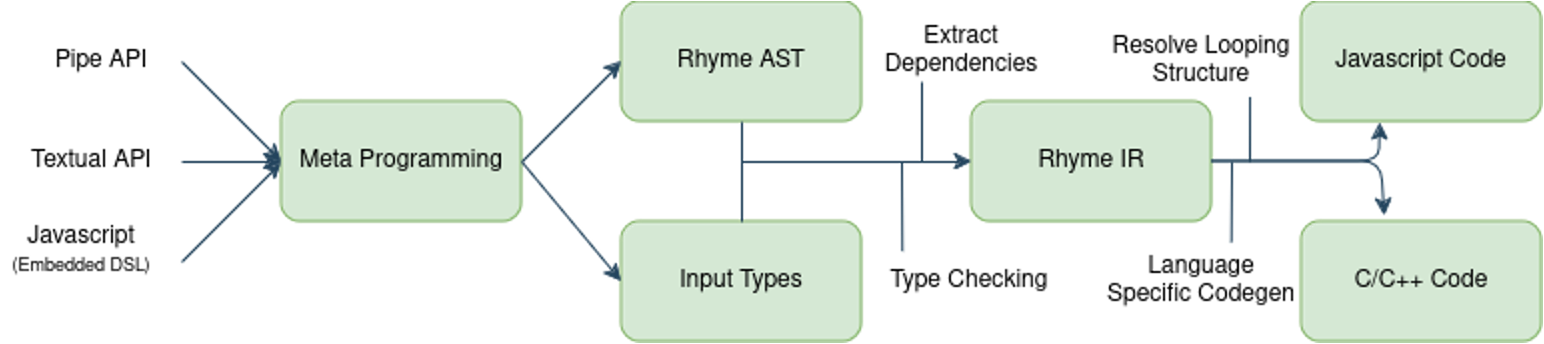
\includegraphics[scale=0.5]{figures/workflow.png}
      \caption{End-to-end workflow of \rhyme}
      \label{workflowfig}
  \end{figure}
\subsection{\rhyme Frontend}
\iffalse
\rhyme has multiple frontends like Pipe API, Textual API and Javascript API. \rhyme is a DSL embedded in Javascript, and as we mentioned before the \rhyme query can itself be a JSON object. Therefore we can use the JSON API to write query where the query is itself a JSON object. For example, if we want to group the sum of values of a dataset by its keys, we can just put \inline{data.*.key} as the key of the object query and put \inline{data.*.value} as the value as shown below. It is worth noting that since the \inline{sum(data.*.value)} is nested with \inline{data.*.key}, the logic variable in \inline{sum(data.*.value)} is bounded, the sum is actually a group-by sum. In addition to JSON API where the user can express the query in the same structure as the results, \rhyme also support Pipe API where the query is expressed as a sequence of transformations. The input wil pass through all the transformations to generate the final results. If we apply the logic variable \inline{.*} to a data source, the input will be iterated and a stream of its data will be passed for the following operation. The pipes are separated by \inline{|} symbol. The JSON API and Pipe API are equivalent and offers different ways to express the query for different application and scenarios. \par
\fi
\rhyme provides multiple frontends, including the Pipe API, Textual API, and JavaScript API. As a domain-specific language (DSL) embedded in JavaScript, \rhyme allows queries to be represented as JSON objects. This design enables users to construct queries directly in JSON format. For instance, to group the sum of values in a dataset by its keys, users can specify \inline{data.*.key} as the object query's key and \inline{data.*.value} as the value, as shown in the example below. Notably, because \inline{sum(data.*.value)} is nested within \inline{data.*.key}, the logic variable in \inline{sum(data.*.value)} is bound, making the operation a group-by sum.

In addition to the JSON API, where queries are expressed in the same hierarchical structure as their results, \rhyme also offers a Pipe API. The Pipe API allows queries to be defined as a sequence of transformations, where the input data passes through each transformation step to produce the final result. By applying the logic variable \inline{.*} to a data source, the input is iterated, and a stream of data is passed to subsequent operations. Transformations in the Pipe API are separated using the \inline{|} symbol.

The JSON API and Pipe API are equivalent in functionality but provide different methods for expressing queries, catering to various applications and scenarios.\par
\vspace*{1pt}
\noindent
\begin{minipage}{0.5\textwidth}\label{jsonapi}
\begin{lstlisting}
// JSON API: group the the sum of values by their keys
let query =  { data.*.key : sum(data.*.value) }
\end{lstlisting}
\end{minipage}%
\begin{minipage}{0.5\textwidth}
\begin{lstlisting}
//  Pipe API: group the sum of values by their keys
let key = rh`.data | .* | .key`
let query = rh`.data | .* | .value | group $\$${key}`
\end{lstlisting}
\end{minipage}
\vspace*{1pt}
\iffalse
The \rhyme query will be first parsed into an AST. The AST is a structured representation of the query and represented using JSON objects. \rhyme AST categorize operations into stateful operations (aggregation) and stateless operations (pure). The keys used for group-by will remain unchanged in the AST node. \rhyme will recursively translate the query into AST nodes and set the operator type and parameter correctly at each level.\par
In order to support generation of strongly typed languages like C/C++, \rhyme also allows user to provide optional type schemas of the input. As shown in Figure \ref{typeschema}, the user specify that the data is an object with u8 (8-bit unsigned integer) keys and string values. This type schema is crucial for our backend code generation as it provides type information for each sub-expressions of the query and allow us to generate more specialized code.
\fi
The \rhyme query is first parsed into an Abstract Syntax Tree (AST), a structured representation of the query expressed as JSON objects. The \rhyme AST categorizes operations into two types: stateful operations (e.g., aggregations) and stateless operations (e.g., pure functions). Keys used for group-by operations remain unchanged within the corresponding AST nodes. The \rhyme compiler recursively translates the query into AST nodes, assigning the appropriate operator types and parameters at each level.

To support code generation for strongly typed languages like C/C++, \rhyme allows users to optionally provide type schemas for the input data. As illustrated in Figure \ref{typeschema}, users can specify, for example, that the data consists of objects with 8-bit unsigned integer (u8) keys and string values. This type schema is essential for backend code generation, as it provides precise type information for each sub-expression of the query, enabling the generation of highly specialized and efficient code. We will talk about the type system more extensively in Section \ref{typesystem}.
\begin{figure}[H]
  \centering
      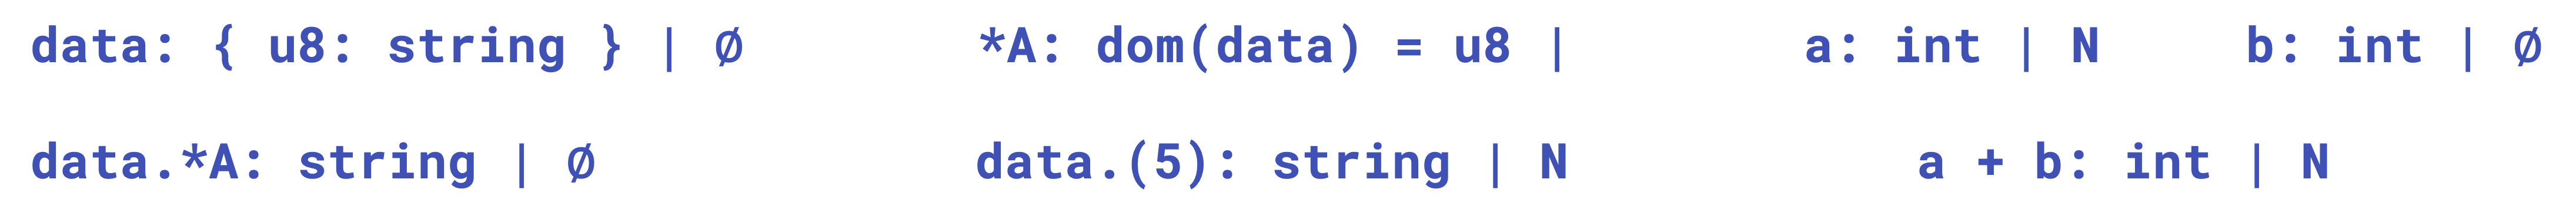
\includegraphics[scale=0.4]{figures/typeschema2.png}
      \caption{Example type schema of \rhyme}
      \label{typeschema}
  \end{figure}
\subsection{\rhyme Middle-end}
\iffalse
After the query is parsed into AST and the type schema is provided, we will perform type checking and inference and generate the intermediate representation. As shown in Figure \ref{typeschema}, we can infer the type of sub-expressions based on the given input type schema. If the input data has type \inline{{u8 : string}}, we can infer that the key of data \inline{*} (i.e. the logic variable) has type u8, we can also infer that \inline{data.*} has type string. We will perform both type inference and type checking to make sure that the type system conforms and we can correctly type all sub-expressions.\par
The \rhyme AST is a structured representation of the query, but we need a more fine-grained representation of the program that can capture both the data and control dependencies.
\rhyme has two types of IRs: \emph{generators} and \emph{assignments}. \emph{generators} are instructions used for iterating over a collection of data. Logic variables are responsible for iterating over data and directly map to generators. For example, \inline{data.*} corresponds to a generator that iterate over \inline{data}. \emph{assignments} are instructions used for computing the final and intermediate results. For example, \inline{sum(data.*)} corresponds to a sum operation that aggregate the value of \inline{data}.\rhyme also utilizes temporary variables to store materialized intermediate results.\par
It is worth noting that the IR does not enforce strict program structures. The program Structure is implied by the dependencies between statements. When an assignment uses a generator, it will cause a generator-assignment dependency (i.e. control dependency). When an assignment uses the result of an intermediate expression, it will cause a assignment-assignment dependency (i.e. data dependency). The \rhyme compiler will utilize these dependencies to produce an optimal program structure that respect the original query's semantic. Due to the dependencies-based IR design, \rhyme can perform multiple optimization like loop hoisting and code motion very easily.\par
After the IR generation, we will also assign types to each IR nodes. We will record the type of each generator and intermediate temporary variables. These type signature will be necessary when we generate code in the backend. We will also record for each generator the type of data sources they are iterating over. And we will generate specialized efficient code to co-iterate multiple data sources for one generator. For example, if one generator is co-iterating over multiple sparse vectors, we can generate specialized code to co-advancing the sparse vectors for efficiency as sparse vector does not offer constant-time look-up. We will cover this more in detail in Section \ref{sparse}.
\fi
After the query is parsed into an AST and the type schema is provided, \rhyme performs type checking and inference, followed by the generation of an intermediate representation (IR). As illustrated in Figure \ref{typeschema}, the type of sub-expressions can be inferred based on the input type schema. For example, if the input data is typed as \inline{\{u8 : string\}}, we can infer that the key of \inline{data} (i.e., the logic variable \inline{*}) has type \inline{u8}, while \inline{data.*} itself has type \inline{string}. Both type inference and type checking ensure that the type system is conformed and that all sub-expressions are correctly typed.

While the \rhyme AST provides a structured representation of the query, it is insufficient for capturing both data and control dependencies. For this purpose, \rhyme introduces two types of IRs: generators and assignments. Generators are instructions for iterating over data collections, with logic variables directly mapping to these generators. For example, \inline{data.*} corresponds to a generator that iterates over \inline{data}. Assignments, on the other hand, represent computations of intermediate and final results. For instance, \inline{sum(data.*)} corresponds to an aggregation operation that computes the sum of \inline{data} values. Temporary variables are also used to store materialized intermediate results.

The \rhyme IR does not enforce a rigid program structure; instead, the structure is implied by the dependencies between statements. A generator used by an assignment introduces a generator-assignment dependency (control dependency), while one assignment using the result of another creates an assignment-assignment dependency (data dependency). These dependencies guide the \rhyme compiler in generating an optimal program structure that preserves the original query semantics. This dependency-based IR design facilitates advanced optimizations such as loop hoisting and code motion.

Following IR generation, types are assigned to each IR node. The compiler records the types of generators and temporary variables, as well as the types of data sources associated with each generator. This type information is critical for backend code generation, enabling specialized and efficient co-iteration of multiple data sources. For example, if a generator co-iterates over multiple sparse vectors, \rhyme generates optimized code for advancing the sparse vectors efficiently, accounting for their lack of constant-time look-up. A more detailed explanation of these optimizations is provided in Section \ref{sparse}.
\subsection{\rhyme Backend}
\section{Type System}\label{typesystem}
\section{Sparse Tensor Algebra}\label{sparse}
\section{Evaluation}\label{evaluation}
\section{Conclusion}\label{conclusion}
%\newpage
\bibliographystyle{acm}
\bibliography{paper}
\end{document}
\endinput
